\documentclass[11pt,a4paper]{article}
%%%----------------------------------------------------------------------------%%%
%%%----------------------------------------------------------------------------%%%
%%% 
%%% ### Packages 
%%%
%%%----------------------------------------------------------------------------%%%
%%%----------------------------------------------------------------------------%%%
\usepackage{amsmath, amsthm, amssymb, nccbbb, bm, dsfont, pifont, fontawesome, graphicx, varioref, enumitem, mathtools, listings, xcolor, cite}
\RequirePackage[round,authoryear]{natbib}
\RequirePackage[colorlinks,citecolor=blue,urlcolor=blue]{hyperref}
\usepackage[cal=boondox]{mathalfa}
%\usepackage[numbers]{natbib}
\setlength{\topmargin}{-1in}
\setlength{\textheight}{10.5in}
\setlength{\oddsidemargin}{-.6in}
\setlength{\textwidth}{7.5in}
\hypersetup{colorlinks=true, linkcolor=blue, citecolor=red, urlcolor=blue}

%%%----------------------------------------------------------------------------%%%
%%%----------------------------------------------------------------------------%%%
%%% 
%%% ### Code 
%%%
%%%----------------------------------------------------------------------------%%%
%%%----------------------------------------------------------------------------%%%
\usepackage{listings}
\lstset{escapeinside=| |}
\usepackage[usenames,dvipsnames]{color}  
\definecolor{mygray}{rgb}{0.99,0.99,0.99}
\definecolor{myblue}{rgb}{0.0, 0.23, 0.63}
\definecolor{myred}{rgb}{0.75, 0.0, 0.0}
\definecolor{mygreen}{rgb}{0.4, 0.69, 0.2}  
\lstnewenvironment{R}{\lstset{ 
  language=R,
  basicstyle=\footnotesize\ttfamily, 
  numbers=left,
  numberstyle=\tiny\color{black},
  stepnumber=1,
  numbersep=5pt,
  backgroundcolor=\color{mygray},
  showspaces=false, 
  showstringspaces=false,
  showtabs=false, 
  frame=single,  
  rulecolor=\color{black},
  tabsize=4,
  captionpos=b,
  breaklines=true,
  breakatwhitespace=false,
  keywordstyle=\ttfamily\bfseries\color{myblue},
  commentstyle=\ttfamily\bfseries\color{myred},
  stringstyle=\ttfamily\bfseries\color{mygreen}
} 
}{}

%New colors defined below
\definecolor{codegreen}{rgb}{0,0.6,0}
\definecolor{codegray}{rgb}{0.5,0.5,0.5}
\definecolor{codepurple}{rgb}{0.58,0,0.82}
\definecolor{backcolour}{rgb}{0.95,0.95,0.92}

%Code listing style named "mystyle"
\lstdefinestyle{mystyle}{
  backgroundcolor=\color{backcolour}, commentstyle=\color{codegreen},
  keywordstyle=\color{magenta},
  numberstyle=\tiny\color{codegray},
  stringstyle=\color{codepurple},
  basicstyle=\ttfamily\footnotesize,
  breakatwhitespace=false,         
  breaklines=true,                 
  captionpos=b,                    
  keepspaces=true,                 
  numbers=left,                    
  numbersep=5pt,                  
  showspaces=false,                
  showstringspaces=false,
  showtabs=false,                  
  tabsize=2
}

%"mystyle" code listing set
\lstset{style=mystyle}

%%%----------------------------------------------------------------------------%%%
%%%----------------------------------------------------------------------------%%%
%%% 
%%% ### Box
%%%
%%%----------------------------------------------------------------------------%%%
%%%----------------------------------------------------------------------------%%%
\usepackage{tcolorbox}
\tcbuselibrary{breakable}
\newtcolorbox{mybox}{colback=yellow!5!white, colframe=gray!60!black, breakable}
\newtcolorbox{mybox0}{colback=white, colframe=gray!60!black, breakable}
	

%%%----------------------------------------------------------------------------%%%
%%%----------------------------------------------------------------------------%%%
%%% 
%%% ### Theorem style structures 
%%%
%%%----------------------------------------------------------------------------%%%
%%%----------------------------------------------------------------------------%%%
\numberwithin{equation}{section}
\theoremstyle{plain}
\newtheorem{theorem}{Theorem}[section]
\newtheorem{lemma}[theorem]{Lemma}
\newtheorem{corollary}[theorem]{Corollary}
\newtheorem{proposition}[theorem]{Proposition}
\newtheorem{condition}{Condition}[section]
\newtheorem{definition}{Definition}[section]
\theoremstyle{definition}
\newtheorem{example}{Example}[section]
\newtheorem{exercise}{Exercise}[section]
\newtheorem{remark}{Remark}[section]
\newtheorem{remark0}{Remark}
\newtheorem{question}{Question}


%%%----------------------------------------------------------------------------%%%
%%%----------------------------------------------------------------------------%%%
%%% 
%%% ### Operators 
%%%
%%%----------------------------------------------------------------------------%%%
%%%----------------------------------------------------------------------------%%%
\newcommand{\pr}{\mathsf{P}} 
\newcommand{\E}{\mathsf{E}} 
\newcommand{\median}{\mathop{\mathsf{median}}}
\newcommand{\Cov}{{\mathsf{Cov}}} 
\newcommand{\Corr}{{\mathsf{Corr}}} 
\newcommand{\Var}{{\mathsf{Var}}}
\newcommand{\SD}{{\mathsf{SD}}}
\newcommand{\CV}{{\mathsf{CV}}}
\newcommand{\Bias}{{\mathsf{Bias}}}
\newcommand{\AMSE}{\operatorname{\mathsf{AMSE}}}
\newcommand{\MSE}{\operatorname{\mathsf{MSE}}}
\newcommand{\ARE}{\mathsf{ARE}}
\newcommand{\AV}{\mathsf{AV}}
\newcommand{\CRLB}{{\mathsf{CRLB}}}

\newcommand{\pCorr}{\text{P}}
\newcommand{\sCorr}{\text{S}}
\newcommand{\kCorr}{\text{K}}
\newcommand{\bdCorr}{\text{BD}}
\newcommand{\cCorr}{\text{C}}


\newcommand{\inD}{    \overset{ \textnormal{d}   }{\rightarrow} }
\newcommand{\inAS}{   \overset{ \textnormal{a.s.}   }{\rightarrow} }
\newcommand{\inP}{    \overset{ \textnormal{pr}    }{\rightarrow} }
\newcommand{\inLp}{   \overset{ \mathcal{L}^p }{\rightarrow} }
\newcommand{\inMSE}{  \overset{ \textnormal{qm} }{\rightarrow} }
\newcommand{\inQM}{   \overset{ \textnormal{qm} }{\rightarrow} }
\newcommand{\indep}{\protect\mathpalette{\protect\independenT}{\perp}}
\def\independenT#1#2{\mathrel{\rlap{$#1#2$}\mkern4mu{#1#2}}}
\newcommand{\iid}{\textsc{iid}} 
\newcommand{\simIID}{   \overset{ \iid   }{\sim} }
\newcommand{\simIND}{   \overset{ {\indep}   }{\sim} }


\newcommand{\Bern}{\textnormal{Bern}} 
\newcommand{\Unif}{\textnormal{Unif}} 
\newcommand{\Normal}{\textnormal{N}} 
\newcommand{\logNormal}{\textnormal{LN}} 
\newcommand{\Bin}{\textnormal{Bin}} 
\newcommand{\NB}{\textnormal{NB}} 
\newcommand{\HG}{\textnormal{HG}} 
\newcommand{\Geom}{\textnormal{Geom}} 
\newcommand{\Beta }{\textnormal{Beta}} 
\newcommand{\BetaBin}{\textnormal{Beta-Bin}}
\newcommand{\Ga}{\textnormal{Ga}} 
\newcommand{\Exp}{\textnormal{Exp}} 
\newcommand{\Expo}{\textnormal{Expo}} 
\newcommand{\Po}{\textnormal{Po}} 
\newcommand{\Multi}{\textnormal{Multi}} 
\newcommand{\student}{\textnormal{t}} 
\newcommand{\Cauchy}{\textnormal{Cauchy}} 
\newcommand{\Pareto}{\textnormal{Pareto}} 
\newcommand{\Laplace}{\textnormal{Laplace}} 
\newcommand{\Logistic}{\textnormal{Logistic}} 
\newcommand{\Dir}{\textnormal{Dir}} 
\newcommand{\DP}{\textnormal{DP}} 
\newcommand{\Inv}{\textnormal{Inv-}} 
\newcommand{\F}{\textnormal{F}} 
\newcommand{\sign}{\textnormal{sign}}
\newcommand{\rank}{\textnormal{rank}}


\newcommand{\RV}{\textsc{rv}}
\newcommand{\cdf}{\textsc{cdf}} 
\newcommand{\cgf}{\textsc{cgf}} 
\newcommand{\pdf}{\textsc{pdf}} 
\newcommand{\pmf}{\textsc{pmf}} 
\newcommand{\chf}{\textsc{chf}} 
\newcommand{\mgf}{\textsc{mgf}}
\newcommand{\EF}{\textsc{EF}}
\newcommand{\NEF}{\textsc{NEF}}
\newcommand{\MLE}{\textsc{mle}}
\newcommand{\MAP}{\textsc{MAP}}
\newcommand{\Med}{\textsc{Med}}
\newcommand{\MME}{\textsc{mme}}
\newcommand{\QME}{\textsc{qme}}
\newcommand{\UMVUE}{\textsc{umvue}}
\newcommand{\MPT}{\textsc{MPT}}
\newcommand{\UMPT}{\textsc{UMPT}}
\newcommand{\LRT}{\textsc{LRT}}


\newcommand{\diag}{\mathop{\mathrm{diag}}}
\newcommand{\tr}{\mathop{\mathrm{tr}}}
\newcommand{\T}{\mathop{\mathrm{T}}}
\DeclareMathOperator*{\argmin}{arg\,min}
\DeclareMathOperator*{\argmax}{arg\,max}
\DeclareMathOperator{\sgn}{sgn}
\DeclareMathOperator{\logit}{logit}
\DeclareMathOperator{\expit}{expit}
\newcommand{\dd}{\textnormal{d}}


\newcommand{\lva}{{\color{myred}\ding{73}\ding{73}\ding{73}}}
\newcommand{\lvb}{{\color{myred}\ding{72}\ding{73}\ding{73}}}
\newcommand{\lvc}{{\color{myred}\ding{72}\ding{72}\ding{73}}}
\newcommand{\lvd}{{\color{myred}\ding{72}\ding{72}\ding{72}}}
\newcommand{\optional}{\noindent{\color{myblue}\faScissors}}
\newcommand{\Solution}{\noindent{\color{myblue}{{\textsc{Solution}}:~$\Big.$}}}
\newcommand{\take}{\noindent{\color{myblue}\faPaperPlaneO~\underline{\bf Takeaway}:~$\Big.$}}

% widecheck 
\DeclareFontFamily{U}{mathx}{\hyphenchar\font45}
\DeclareFontShape{U}{mathx}{m}{n}{
      <5> <6> <7> <8> <9> <10>
      <10.95> <12> <14.4> <17.28> <20.74> <24.88>
      mathx10
      }{}
\DeclareSymbolFont{mathx}{U}{mathx}{m}{n}
\DeclareFontSubstitution{U}{mathx}{m}{n}
\DeclareMathAccent{\widecheck}{0}{mathx}{"71}
\DeclareMathAccent{\wideparen}{0}{mathx}{"75}

\def\cs#1{\texttt{\char`\\#1}}

\newcounter{magicrownumbers}
\newcommand\rownumber{\stepcounter{magicrownumbers}\arabic{magicrownumbers}}

\usepackage[table]{xcolor}
%------------------------------------------------------------------------------



\begin{document}
    % Page 0 for names and table of contents
    \thispagestyle{empty}
    \pagenumbering{gobble} 
    \title{\textsc{RMSC 4002} -- Financial Data Analytics with Machine Learning \\ Group Project}
    \author{
        CHOI Sen Hei (SID: \texttt{1155109412}) \\
        IEONG Hei (SID: \texttt{1155104271}) \\
        LAM Wai Chui (SID: \texttt{1155152095}) \\
        LAU Chiu Tan (SID: \texttt{1155108960}) \\
        LAW Yiu Leung Eric (SID: \texttt{1155149315})
    }
    \date{\today}
    \maketitle
    
    \tableofcontents
    \newpage
    
    
    % Section 1
    \pagenumbering{arabic}
    \setcounter{page}{1}
    
    % \section{Principal Component Analysis Factor Models and Recommender Systems}
    \section{Principal Component Analysis Factor Models}
    \textbf{This section is contributed by CHOI Sen Hei (SID: 1155109412), IEONG Hei (SID: 1155104271) and LAU Chiu Tan (SID: 1155108960).}
    
    \subsection{Pricipal Component Analysis (PCA)}
    
    
    % Section 2
    \newpage
    \section{Classification / Decision and Regression Trees}
    \textbf{This section is contributed by LAM Wai Chui (SID: 1155152095) and LAW Yiu Leung Eric (SID: 1155149315)}. \\
    In this section, we are going to use Decision Tree and Random Forest methods to predict binary response variable. The source code is attached in \texttt{src/python/classification.ipynb}, notice that the output in this written report may be slightly different with the python notebook, due to random seed is involved.
    
    \subsection{Dataset}
    For the dataset, we use \href{https://archive.ics.uci.edu/ml/datasets/bank+marketing}{Bank Marketing Data Set} from  \href{https://archive.ics.uci.edu/ml/index.php}{UCI Machine Learning Repository}.
    The data is related with direct marketing campaigns of a Portuguese banking institution. The marketing campaigns were based on phone calls. Often, more than one contact to the same client was required, in order to access if the product (bank term deposit) would be ('yes') or not ('no') subscribed \cite{MORO201422}. There are total 21 variables (including y, the response variable), 41188 valid records. \\
    
    \noindent
    \textbf{Samples of the dataset:}
    \begin{table}[ht]
        \centering
        \begin{tabular}{lrlllllllcl}
            {} &  age &          job &   marital &          education & default & housing & loan &   contact & ... & y\\
            
            \hline \hline
            
            35666 &   58 &   management &   married &  university.degree &      no &      no &   no &  cellular & ... & no \\
            36531 &   48 &       admin. &   married &  university.degree &      no &     yes &   no &  cellular & ... & yes \\
            38676 &   73 &      retired &   married &  university.degree &      no &      no &  yes &  cellular & ... & yes \\
            15146 &   49 &   technician &  divorced &        high.school &      no &      no &   no &  cellular & ... & no \\
            33230 &   33 &  blue-collar &    single &           basic.6y &      no &     yes &   no &  cellular & ... & no \\
        \end{tabular} \\ \\
        \caption{Dataset Samples}
        \label{tab:samples}
    \end{table}
    
    \noindent
    There are 41188 observations with 21 features
    % \begin{tabular}{lrlllllllcl}
    %     {} &  age &          job &   marital &          education & default & housing & loan &   contact & ... & y\\
        
    %     35666 &   58 &   management &   married &  university.degree &      no &      no &   no &  cellular & ... & no \\
    %     36531 &   48 &       admin. &   married &  university.degree &      no &     yes &   no &  cellular & ... & yes \\
    %     38676 &   73 &      retired &   married &  university.degree &      no &      no &  yes &  cellular & ... & yes \\
    %     15146 &   49 &   technician &  divorced &        high.school &      no &      no &   no &  cellular & ... & no \\
    %     33230 &   33 &  blue-collar &    single &           basic.6y &      no &     yes &   no &  cellular & ... & no \\
    % \end{tabular} \\ \\
    % There are 41188 observations with 21 features
    
    
    \subsection{Feature Description}
    There are 20 explanatory variables, including numerical and categorical variables:
    
    \begin{table}[h]
        \begin{minipage}{.5\linewidth}
            \centering
            \begin{tabular}{r c c}
                 & Feature & Type \\
                \hline \hline
                \rownumber & age & numerical \\
                \rownumber & job & categorical \\
                \rownumber & marital & categorical \\
                \rownumber & education & categorical \\
                \rownumber & default & categorical \\
                \rownumber & housing & categorical \\
                \rownumber & loan & categorical \\
            \end{tabular}
            \caption{Bank client data}\label{tab:bank.client}
        \end{minipage}%
        \begin{minipage}{.5\linewidth}
            \centering
            \begin{tabular}{r c c}
                 & Feature & Type \\
                \hline \hline
                \rownumber & contact & categorical \\
                \rownumber & month & categorical \\
                \rownumber & day\_of\_week & categorical \\
                \rownumber & duration & numerical \\
            \end{tabular}
            \caption{Related with the last contact of the current campaign}\label{tab:last.contact}
        \end{minipage}
    \end{table}
    
    \begin{table}[h]
        \begin{minipage}{.5\linewidth}
            \centering
            \begin{tabular}{r c c}
                 & Feature & Type \\
                \hline \hline
                \rownumber & campaign & numerical \\
                \rownumber & pdays & numerical \\
                \rownumber & previous & numerical \\
                \rownumber & poutcome & categorical \\
            \end{tabular}
            \caption{Other attributes}\label{tab:other}
        \end{minipage}%
        \begin{minipage}{.5\linewidth}
            \centering
            \begin{tabular}{r c c}
                 & Feature & Type \\
                \hline \hline
                \rownumber & emp.var.rate & numerical \\
                \rownumber & cons.price.idx & numerical \\
                \rownumber & cons.conf.idx & numerical \\
                \rownumber & euribor3m & numerical \\
                \rownumber & nr.employed & numerical \\
            \end{tabular}
            \caption{social and economic context attributes}\label{tab:soc.econ}
        \end{minipage}
    \end{table}
    
    \newpage
    \subsection{Project Description}
    We are going to perform an analysis in \textbf{topic 6: Classification / Decision and Regression Trees}. We will use \nameref{decision_trees}, \nameref{random_forest} and also \nameref{logistic_regression} to do classification on response variable \textbf{y}, i.e. whether the client subscribed a term deposit. \\
    
    
    \noindent
    The following steps will be performed to complete this section:
    \begin{enumerate}
        \item process data explanatory data analysis (EDA)
        \item data preparation for modeling
        \item visualization of random forest, decision tree and logistic regression
        \item cross validation and grid search
        \item logistic regression
        \item comparison of performance of random forest, decision tree and logistic regression
        \item conclusion
    \end{enumerate}
    
    \subsection{Process Data and Explanatory Data Analysis (EDA)}
%     Import libraries
% \begin{lstlisting}[language = Python]
% import pandas as pd
% import numpy as np
% from datetime import datetime
% import time
% import gc
% from IPython.display import display
% import warnings
% warnings.filterwarnings("ignore")

% from sklearn.model_selection import train_test_split, GridSearchCV, StratifiedKFold
% from sklearn.ensemble import RandomForestClassifier
% from sklearn import tree
% from sklearn.pipeline import Pipeline
% from sklearn.metrics import roc_curve, roc_auc_score
% import category_encoders as ce

% import plotly.graph_objs as go
% import matplotlib.pyplot as plt
% \end{lstlisting}

    % \noindent
    In order to easily implement machine learning algorithms, instead of writing from scratch, we imported \texttt{sklearn} library \cite{sklearn_api}.
    
%     \noindent Loading data and a short explanatory data analysis
% \begin{lstlisting}[language = Python]
% # Process data
% data = pd.read_csv('../../data/bank-additional-full.csv', sep=';')
% display(data.sample(10))
% display('There are {} observations with {} features'.format(data.shape[0], data.shape[1]))
% \end{lstlisting}
    
    
    
    \subsubsection{Categorical Variables}
% \begin{lstlisting}[language = Python]
% # Function of plotting the categorical values disribution
% def plot_bar(column):
%     temp = pd.DataFrame()  #create a tremp dataframe
%     temp['Not_deposit'] = data[data['y'] == 'no'][column].value_counts() # count the value when y = no
%     temp['Deposit'] = data[data['y'] == 'yes'][column].value_counts() # count the value when y = yes

%     temp = temp.apply(lambda x: x / x.sum(), axis = 1) * 100
%     temp.sort_values("Deposit", inplace = True)
%     temp.plot(
%         kind = "barh", 
%         stacked = True, 
%         title = "Percentage Stacked Bar Graph for {}".format(column), 
%         mark_right = True
%     ).legend(loc = "center left", bbox_to_anchor = (1, 0.5))

%     plt.savefig("../../plot/classification/{}.pdf".format(column), bbox_inches = "tight")
%     plt.show();

% plot_bar('job'), plot_bar('marital'), plot_bar('education'), plot_bar('contact'), plot_bar('loan'), plot_bar('housing')
% \end{lstlisting}
    
    We plot percentage stacked bar graphs for 6 categorical variables in table \ref{tab:bank.client} vs. \texttt{y}, to see the proportions of \texttt{y} = 1 given the client is different categories.
    
    \noindent
    \begin{figure}[H]
        \centering
        \subfloat[job]{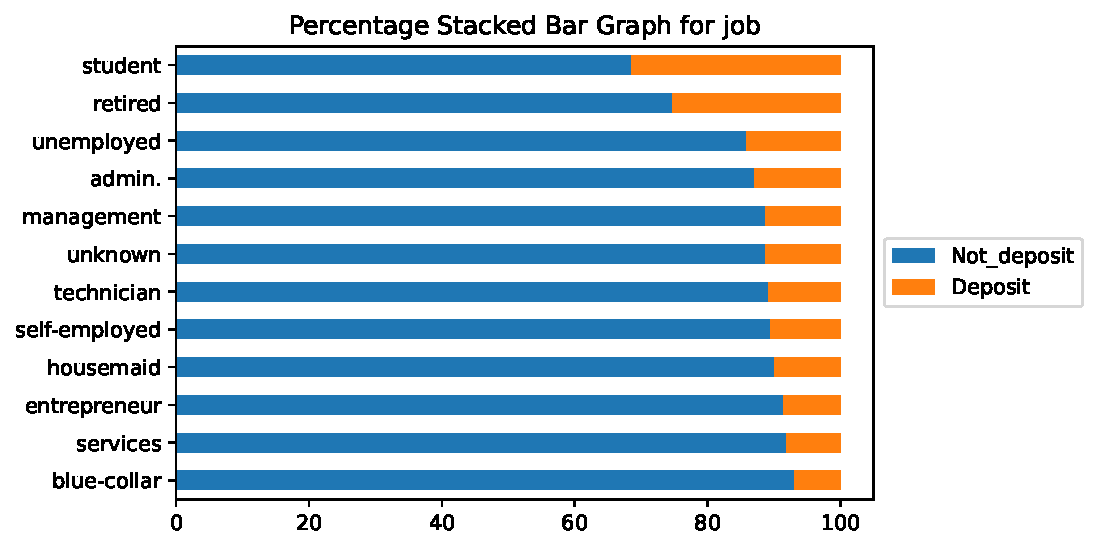
\includegraphics[scale=0.4]{plot/classification/job.pdf}}%
        \qquad
        \subfloat[marital]{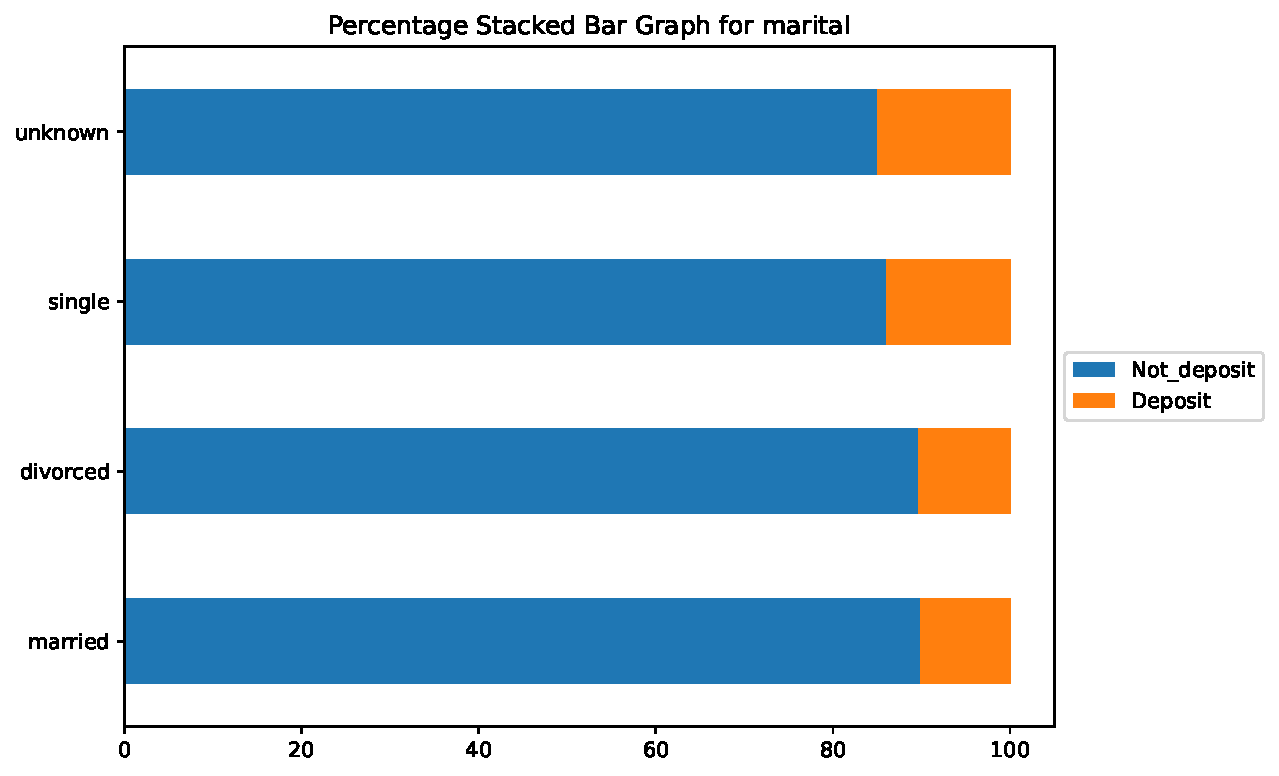
\includegraphics[scale=0.4]{plot/classification/marital.pdf}}%
    
        \subfloat[education]{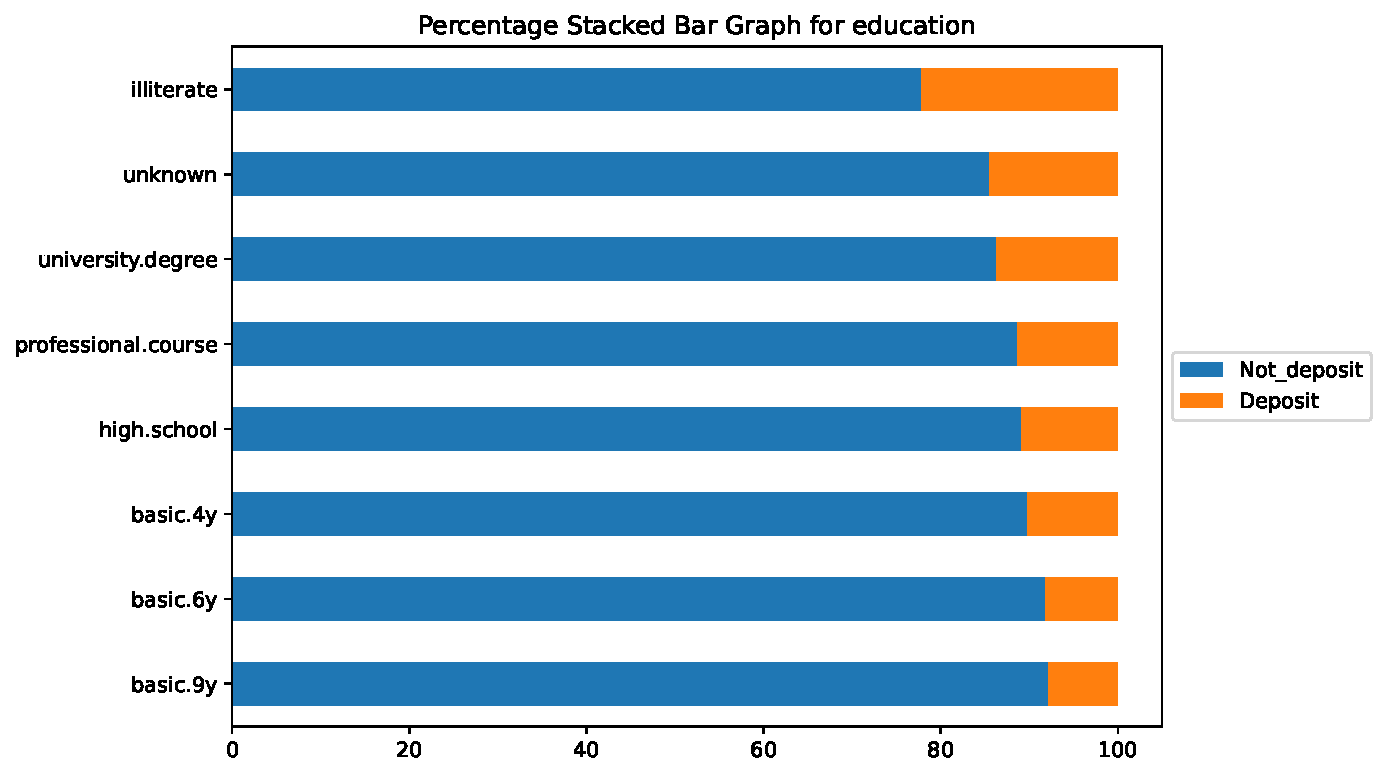
\includegraphics[scale=0.4]{plot/classification/education.pdf}}%
        \qquad
        \subfloat[contact]{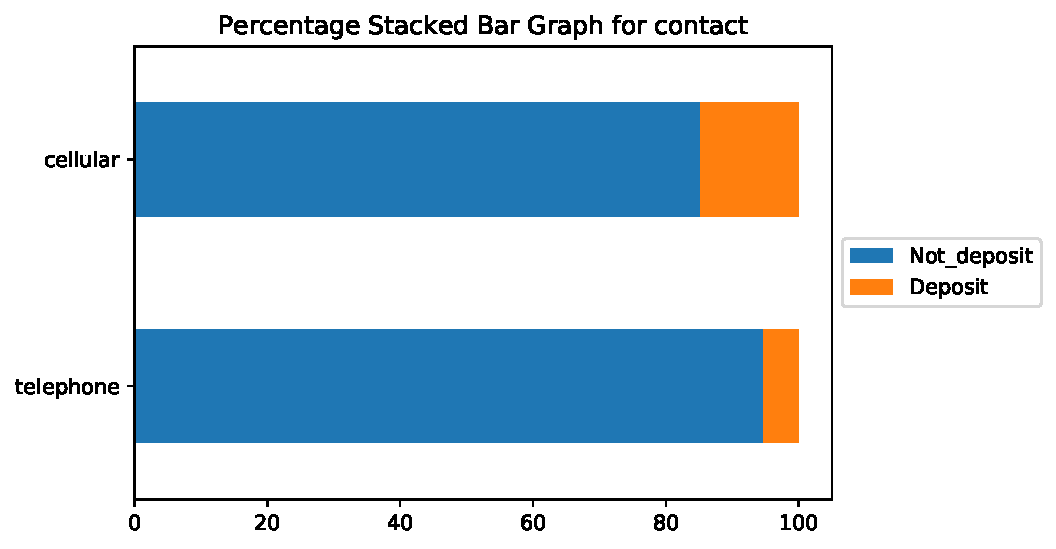
\includegraphics[scale=0.4]{plot/classification/contact.pdf}}%
        
        % \subfloat[loan]{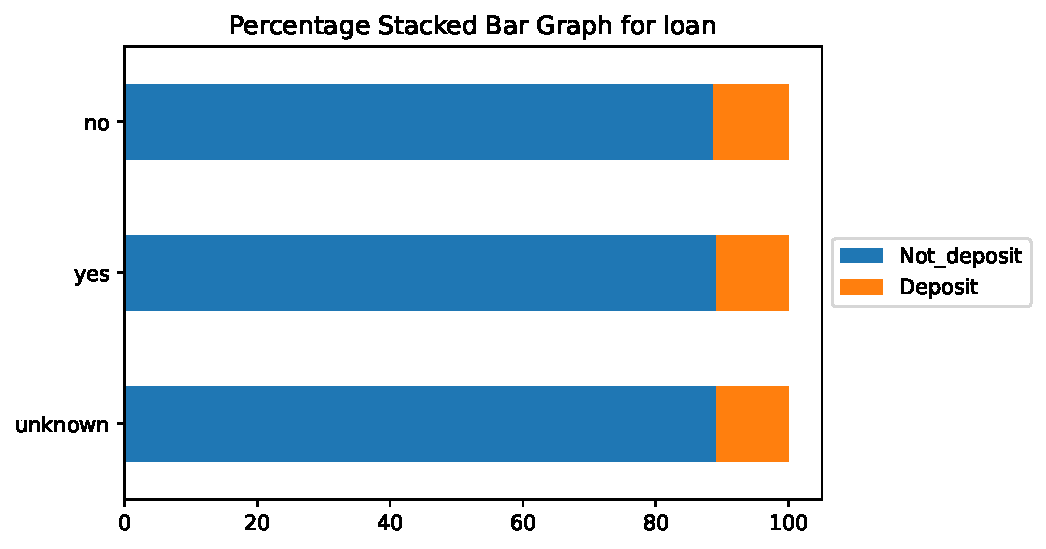
\includegraphics[scale=0.4]{plot/classification/loan.pdf}}%
        % \qquad
        % \subfloat[contact]{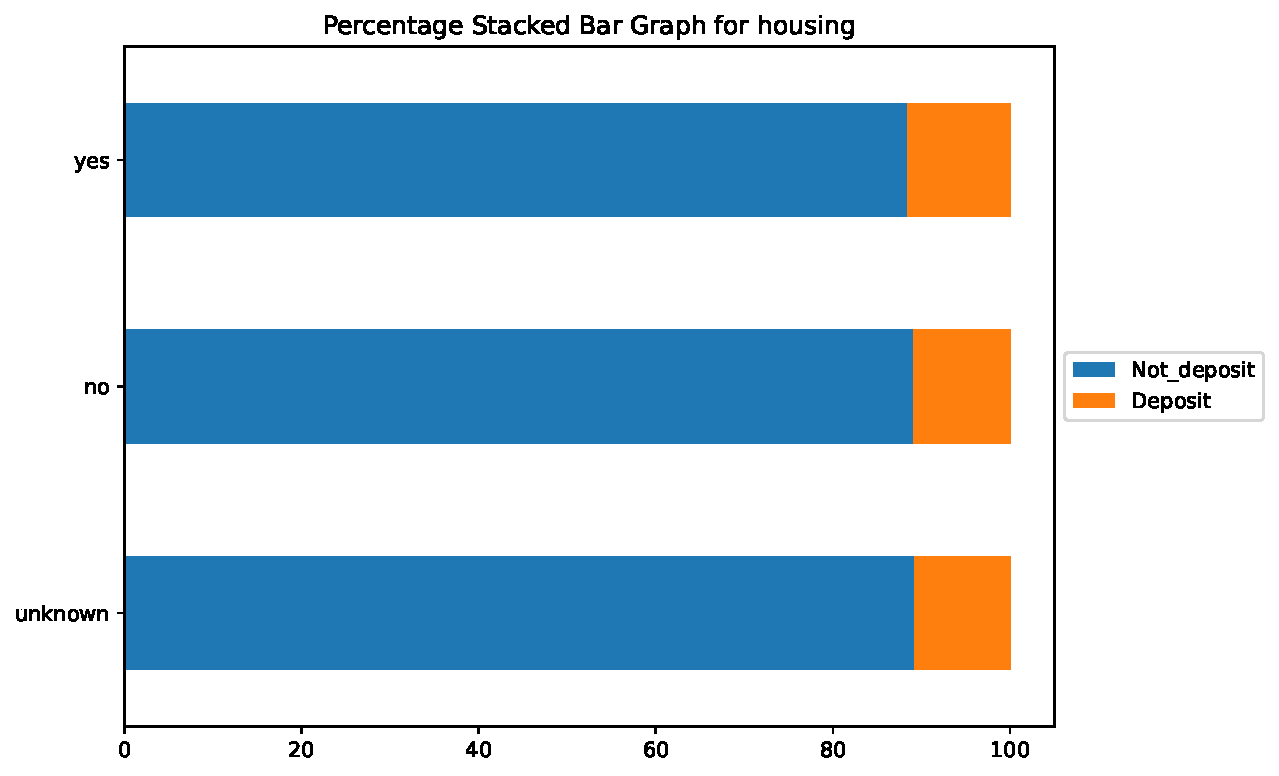
\includegraphics[scale=0.4]{plot/classification/housing.pdf}}%
    \end{figure}
    
        \begin{figure}[H]
        \centering
        % \subfloat[job]{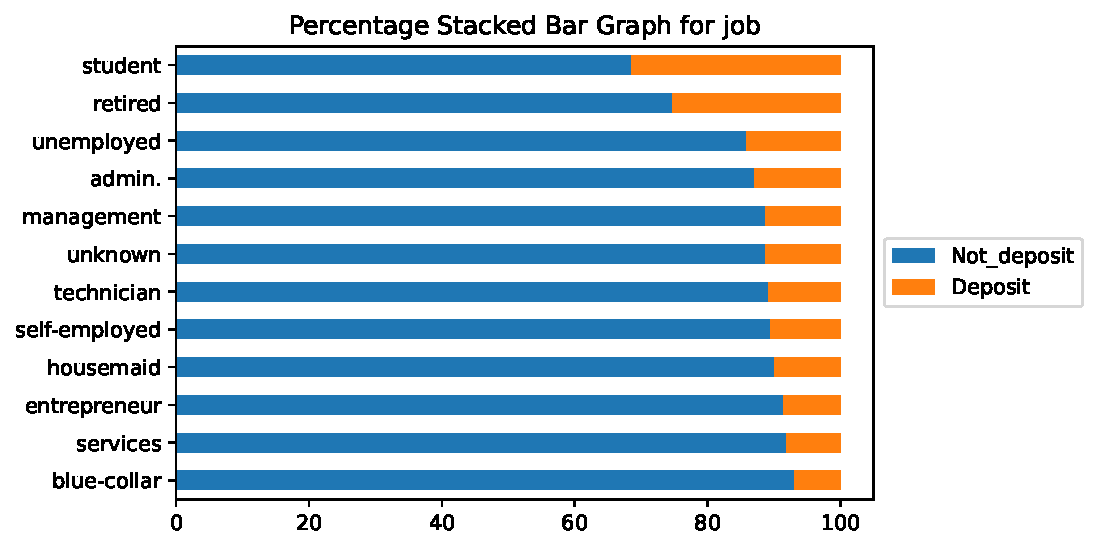
\includegraphics[scale=0.4]{plot/classification/job.pdf}}%
        % \qquad
        % \subfloat[marital]{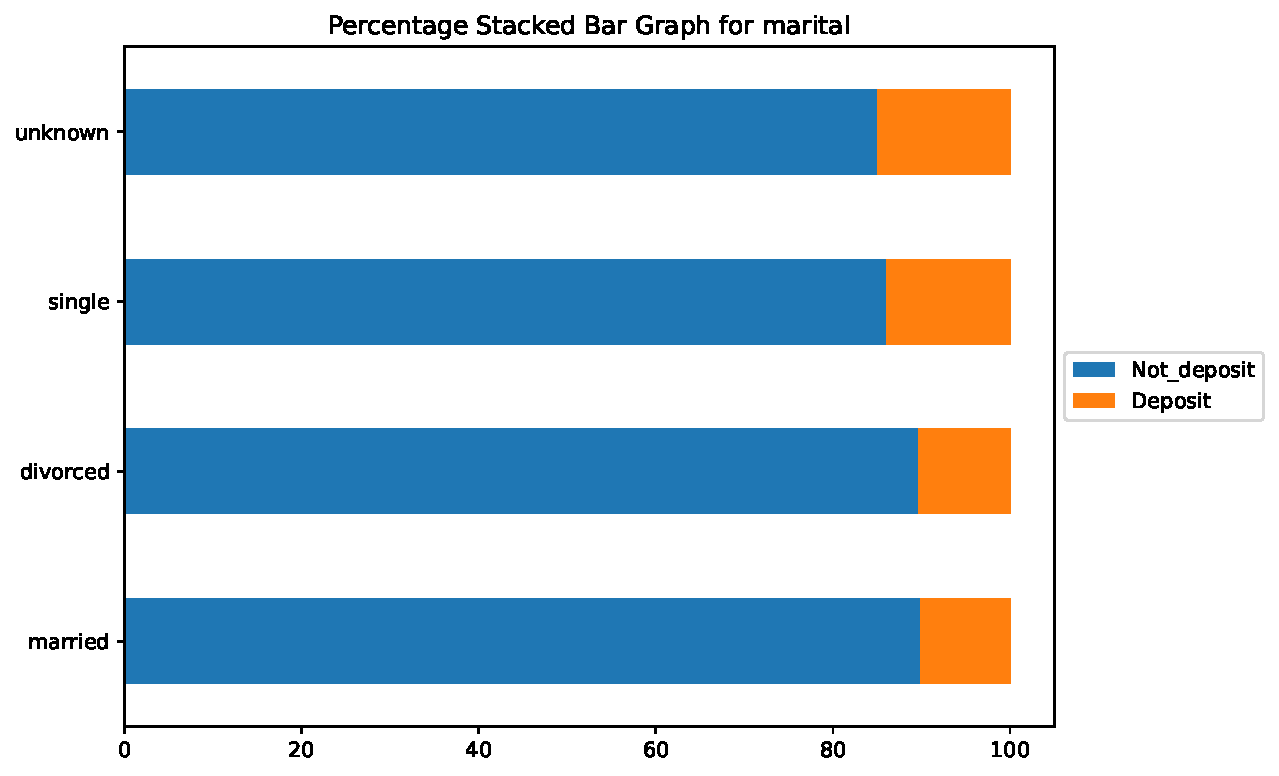
\includegraphics[scale=0.4]{plot/classification/marital.pdf}}%
    
        % \subfloat[education]{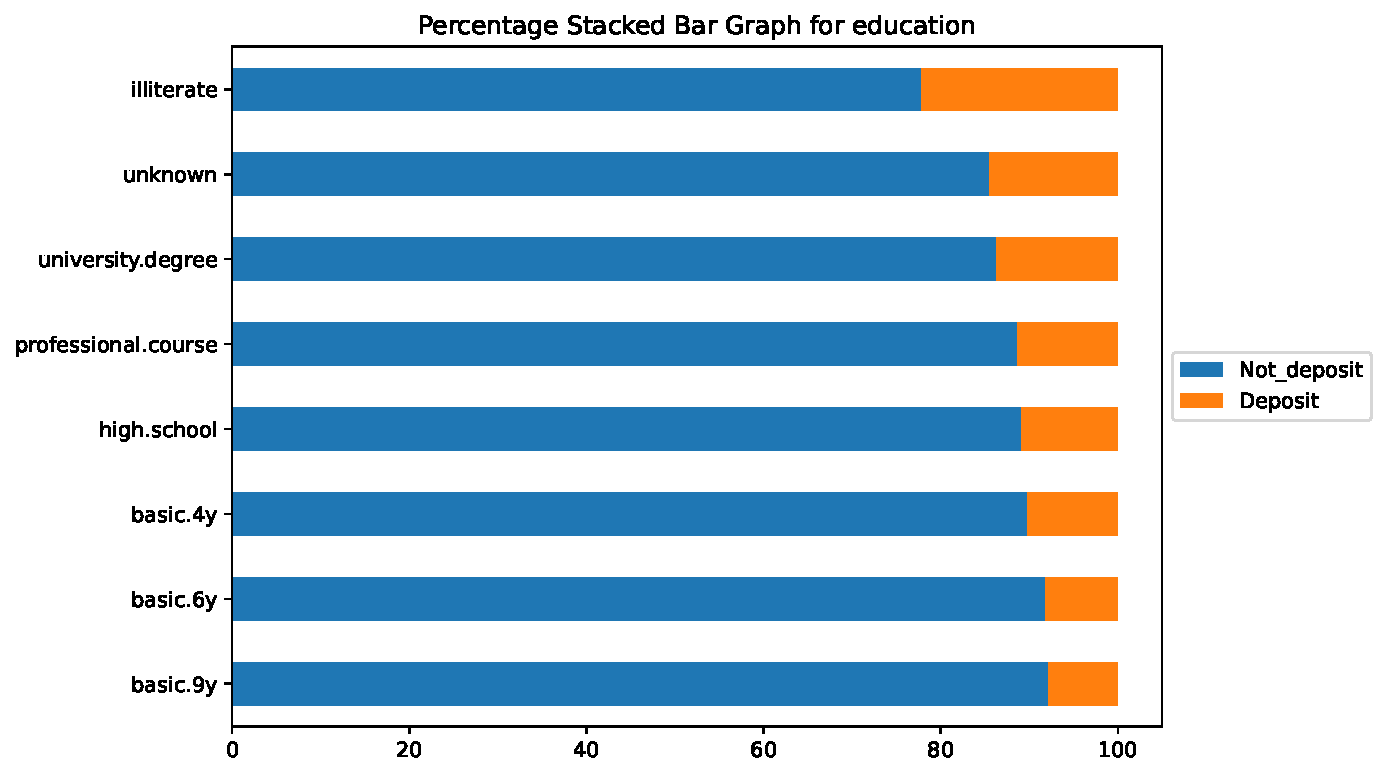
\includegraphics[scale=0.4]{plot/classification/education.pdf}}%
        % \qquad
        % \subfloat[contact]{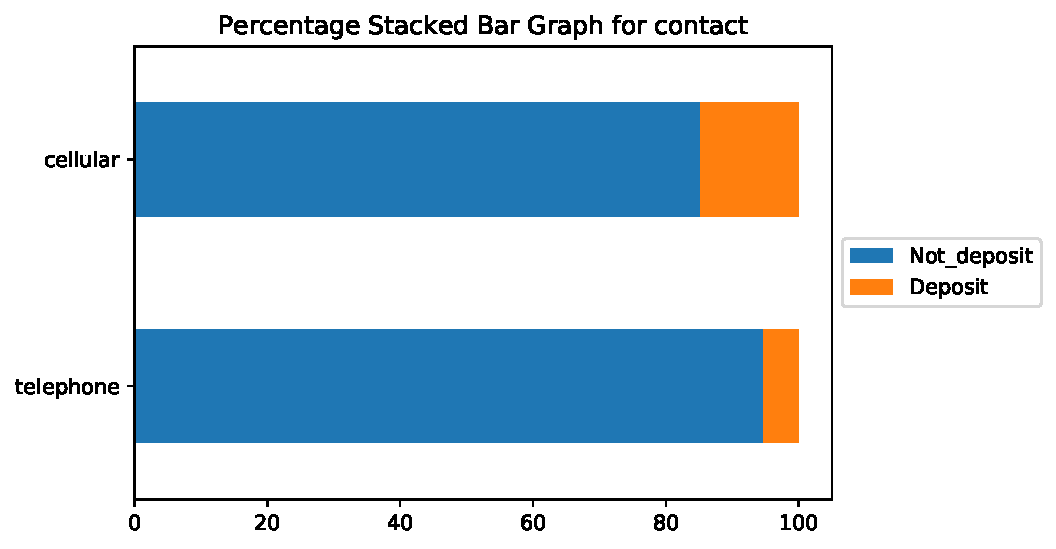
\includegraphics[scale=0.4]{plot/classification/contact.pdf}}%
        
        \subfloat[loan]{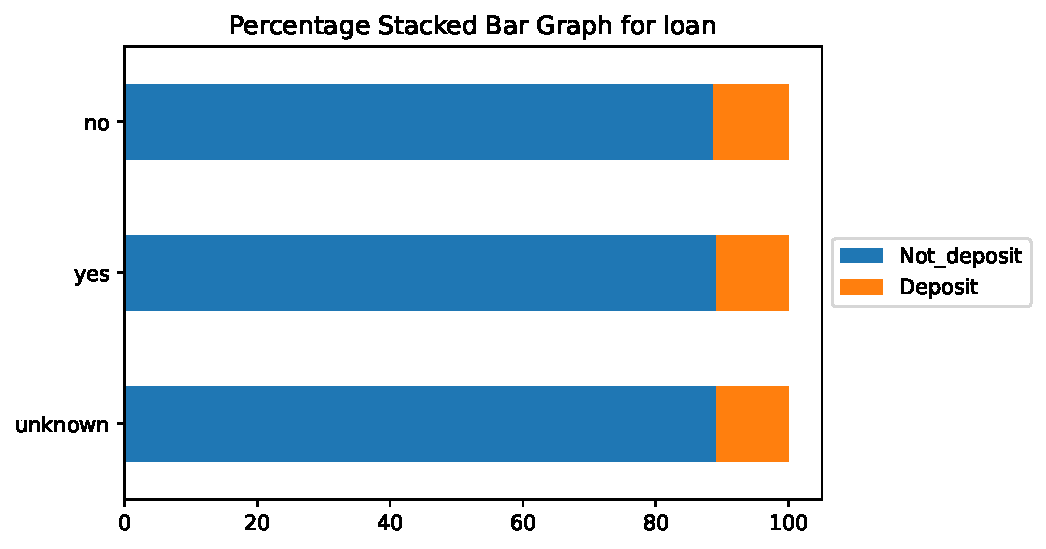
\includegraphics[scale=0.4]{plot/classification/loan.pdf}}%
        \qquad
        \subfloat[contact]{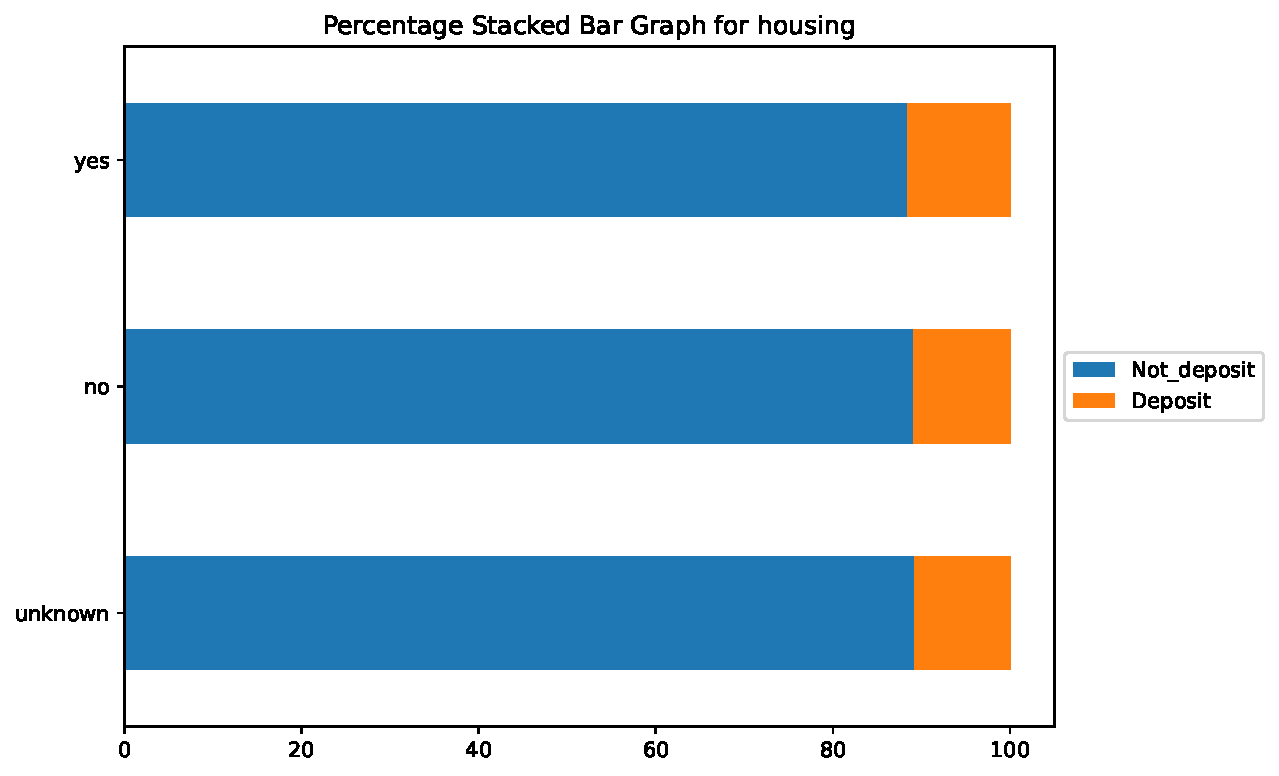
\includegraphics[scale=0.4]{plot/classification/housing.pdf}}%
    \end{figure}
    
    
    
    \noindent \textbf{Summary of Categorical Variables:}
    \begin{enumerate}
        \item 
            The proportion of opening deposit or not is different among different job type. When the job types are student, retired and unemployed, the proportions of opening the deposit are highest. When the job types are entrepreneur, services and blue-collar, the proportions of opening the deposit are lowest.
        
        \item
            The proportion of opening deposit of unknown is close to that of single, while both of them have higher proportion than divorced and married.
        
        \item
            It is surprised to see that illiterate has the highest proportion, other than that, generally higher education levels have higher proportion of opening deposit.
            
        \item
            The proportion of opening deposit of using cellular is much higher than that of using telephone.
            
        \item
            The proportion is basically no different among loan status.
            
        \item
            The proportion is basically no different among contact status.
    \end{enumerate}
    
    \subsubsection{Numerical Variables}
% \begin{lstlisting}[language = Python]
% corr = data.corr()
% corr.style.background_gradient(cmap = 'Spectral')
% \end{lstlisting}
    After exploring the categorical variables, we take a look into numerical variables, by calculate (Pearson) correlations of each variables, we can see which variables have significant relationship with \texttt{y}. The correlation matrix are as follow: 
    \begin{table}[h]
        \centering
        {\tiny
            \begin{tabular}{l||rrrrrrrrrrr}
                {} &     age &  duration &  campaign &   pdays &  previous &  emp.var.rate &  cons.price.idx &  cons.conf.idx &  euribor3m &  nr.employed &       y \\
                \hline \hline
                age            &  1.0000 &   -0.0009 &    0.0046 & -0.0344 &    0.0244 &       -0.0004 &          0.0009 &         0.1294 &     0.0108 &      -0.0177 &  0.0304 \\
                duration       & -0.0009 &    1.0000 &   -0.0717 & -0.0476 &    0.0206 &       -0.0280 &          0.0053 &        -0.0082 &    -0.0329 &      -0.0447 &  0.4053 \\
                campaign       &  0.0046 &   -0.0717 &    1.0000 &  0.0526 &   -0.0791 &        0.1508 &          0.1278 &        -0.0137 &     0.1351 &       0.1441 & -0.0664 \\
                pdays          & -0.0344 &   -0.0476 &    0.0526 &  1.0000 &   -0.5875 &        0.2710 &          0.0789 &        -0.0913 &     0.2969 &       0.3726 & -0.3249 \\
                previous       &  0.0244 &    0.0206 &   -0.0791 & -0.5875 &    1.0000 &       -0.4205 &         -0.2031 &        -0.0509 &    -0.4545 &      -0.5013 &  0.2302 \\
                emp.var.rate   & -0.0004 &   -0.0280 &    0.1508 &  0.2710 &   -0.4205 &        1.0000 &          0.7753 &         0.1960 &     0.9722 &       0.9070 & -0.2983 \\
                cons.price.idx &  0.0009 &    0.0053 &    0.1278 &  0.0789 &   -0.2031 &        0.7753 &         1.0000 &         0.0590 &     0.6882 &       0.5220 & -0.1362 \\
                cons.conf.idx  &  0.1294 &   -0.0082 &   -0.0137 & -0.0913 &   -0.0509 &        0.1960 &          0.0590 &         1.0000 &     0.2777 &       0.1005 &  0.0549 \\
                euribor3m      &  0.0108 &   -0.0329 &    0.1351 &  0.2969 &   -0.4545 &        0.9722 &          0.6882 &         0.2777 &     1.0000 &       0.9452 & -0.3078 \\
                nr.employed    & -0.0177 &   -0.0447 &    0.1441 &  0.3726 &   -0.5013 &        0.9070 &          0.5220 &         0.1005 &     0.9452 &       1.0000 & -0.3547 \\
                y              &  0.0304 &    0.4053 &   -0.0664 & -0.3249 &    0.2302 &       -0.2983 &         -0.1362 &         0.0549 &    -0.3078 &      -0.3547 &  1.0000 \\
            \end{tabular}
        }
        \caption{Correlation Matrix}
        \label{tab:corr_mat}
    \end{table}

    \noindent
    \textbf{Summary of Numerical Variables:}
    \begin{itemize}
        \item \texttt{duration} is the highest correlated variable with target feature (0.4053).
        \item \texttt{nr.employed, pdays, euribor3m} are also highly correlated with target feature.
    \end{itemize}
    
    
    \newpage
    \subsection{Data Preparation for modeling}
    \subsubsection{Transformation for Categorical Variables}
    Since this dataset contains a lot of categorical variables and the number of weakly correlated numeric variables is small, therefore, we use one-hot encoding to transform categorical data.
    \begin{itemize}
        \item 
            For binary categorical variables (\texttt{"yes", "no"}), we transform it into binary number accordingly (\texttt{0, 1}).
            
        \item
            For \texttt{job, marital, education, month, day\_of\_week}, we use one-hot encoding to transform these variables since they have more than 3 types of possible options. Also, some variables contain missing data, labeled as \texttt{unknown} or \texttt{nonexistent}, we treat it as 0 (i.e. no) in general.
        
        \item
            For \texttt{pdays}, there exists many records of \texttt{999} which means the client was not previously contacted, we replaces those with \texttt{0}.
        
        \item
            At last, we remove duplicated records.
    \end{itemize}

    
    
% \begin{lstlisting}[language = Python]
% # Fucntion of One Hot Encoding
% def encode(data, col):
%     return pd.concat([data, pd.get_dummies(col, prefix=col.name)], axis=1)

% # Replacing values with binary number
% data.contact = data.contact.map({'cellular': 0, 'telephone': 1}).astype('uint8') 
% data.loan = data.loan.map({'unknown': 0, 'no' : 0, 'yes': 1}).astype('uint8')
% data.default = data.default.map({'unknown': 0,'no': 0, 'yes': 1}).astype('uint8')
% data.housing = data.housing.map({'unknown': 0, 'no' : 0,'yes': 1}).astype('uint8')
% # binary if were was an outcome of marketing campane
% data.poutcome = data.poutcome.map({'nonexistent':0, 'failure':0, 'success':1}).astype('uint8') 

% # One Hot encoding of 3 variable 
% data = encode(data, data.job)
% data = encode(data, data.month)
% data = encode(data, data.day_of_week)

% # Drop tranfromed features
% data.drop(['job','month', 'day_of_week'], axis=1, inplace=True)

% '''Drop the dublicates'''
% data.drop_duplicates(inplace=True) 

% # Save target variable as y
% y = data.y
% # Create target encoder object and transoform marital and education
% target_encode = ce.target_encoder.TargetEncoder(cols=['marital', 'education']).fit(data, y)
% dataset_prepared = target_encode.transform(data)
% # Drop target variable
% dataset_prepared.drop('y', axis=1, inplace=True)

% display(dataset_prepared.sample(10))
% display('There are {} observations with {} features in the prepared dataset'.format(dataset_prepared.shape[0], dataset_prepared.shape[1]))
% \end{lstlisting}
    % \noindent
    \begin{table}[ht]
        \centering
        \begin{tabular}{lrrrrrrrrrc}
            {} &  age &   marital &  education &  default &  housing &  loan &  contact &  duration &  campaign & \dots \\
            \hline \hline
            29851 &   52 &  0.103231 &   0.137219 &        0 &        1 &     0 &        1 &        70 &         4 & \dots \\
            15768 &   39 &  0.140090 &   0.113550 &        0 &        0 &     0 &        0 &        65 &         2 & \dots \\
            38033 &   76 &  0.101569 &   0.102515 &        0 &        1 &     0 &        0 &       259 &         2 & \dots \\
            27290 &   37 &  0.140090 &   0.137219 &        0 &        1 &     1 &        0 &       661 &         1 & \dots \\
            30685 &   34 &  0.101569 &   0.078246 &        0 &        1 &     0 &        0 &       332 &         1 & \dots \\
        \end{tabular}
        \caption{Dataset Samples after Encoding}
        \label{tab:samples_encoded}
    \end{table}
    
    \noindent
    After removing duplicates, there are 41173 observations with 44 features in the prepared dataset
    
    
    \subsubsection{Splitting Training Dataset and Testing Dataset}
    To test the performance of machine learning alogrithm, we split the dataset into training and testing datasets, 80\% and 20\% of the full dataset respectively. The models would be built using training dataset, and evaluated the performance using testing dataset accordingly. In order to make the prediction model reproducible, we fixed the random seed: \texttt{random\_state=4002}. \\
    Total records in training dataset = 32938, number of class \texttt{0} and \textt{1} in training dataset: \texttt{[29267, 3671]}, noted that this is the numbers of true positive and true negative. These are used to calculate the support, confidence and capture in evaluating performance under training dataset.
% \begin{lstlisting}[language = Python]
% # Set global random seed
% random_state = 4002
% # split data
% x_train, x_test, y_train, y_test = train_test_split(dataset_prepared, y, test_size=0.2, random_state=random_state)
% \end{lstlisting}
    
    
    \newpage
    \subsection{Decision Tree} \label{decision_trees}
    We set the depth of decision tree to 3, in order to plot a simplified decision tree.
% \begin{lstlisting}[language = Python]
% # Set max_depth = 3 to keep the size of the tree small for ploting graph
% dt = tree.DecisionTreeClassifier(max_depth=3, random_state=random_state)
% dt.fit(x_train, y_train)
% plt.figure(figsize=(10, 5))
% _ = tree.plot_tree(dt, feature_names=dataset_prepared.columns,
%                   class_names=["0", "1"], filled=True)
% \end{lstlisting}

    % \noindent
    \begin{figure}[ht]
        \centering
        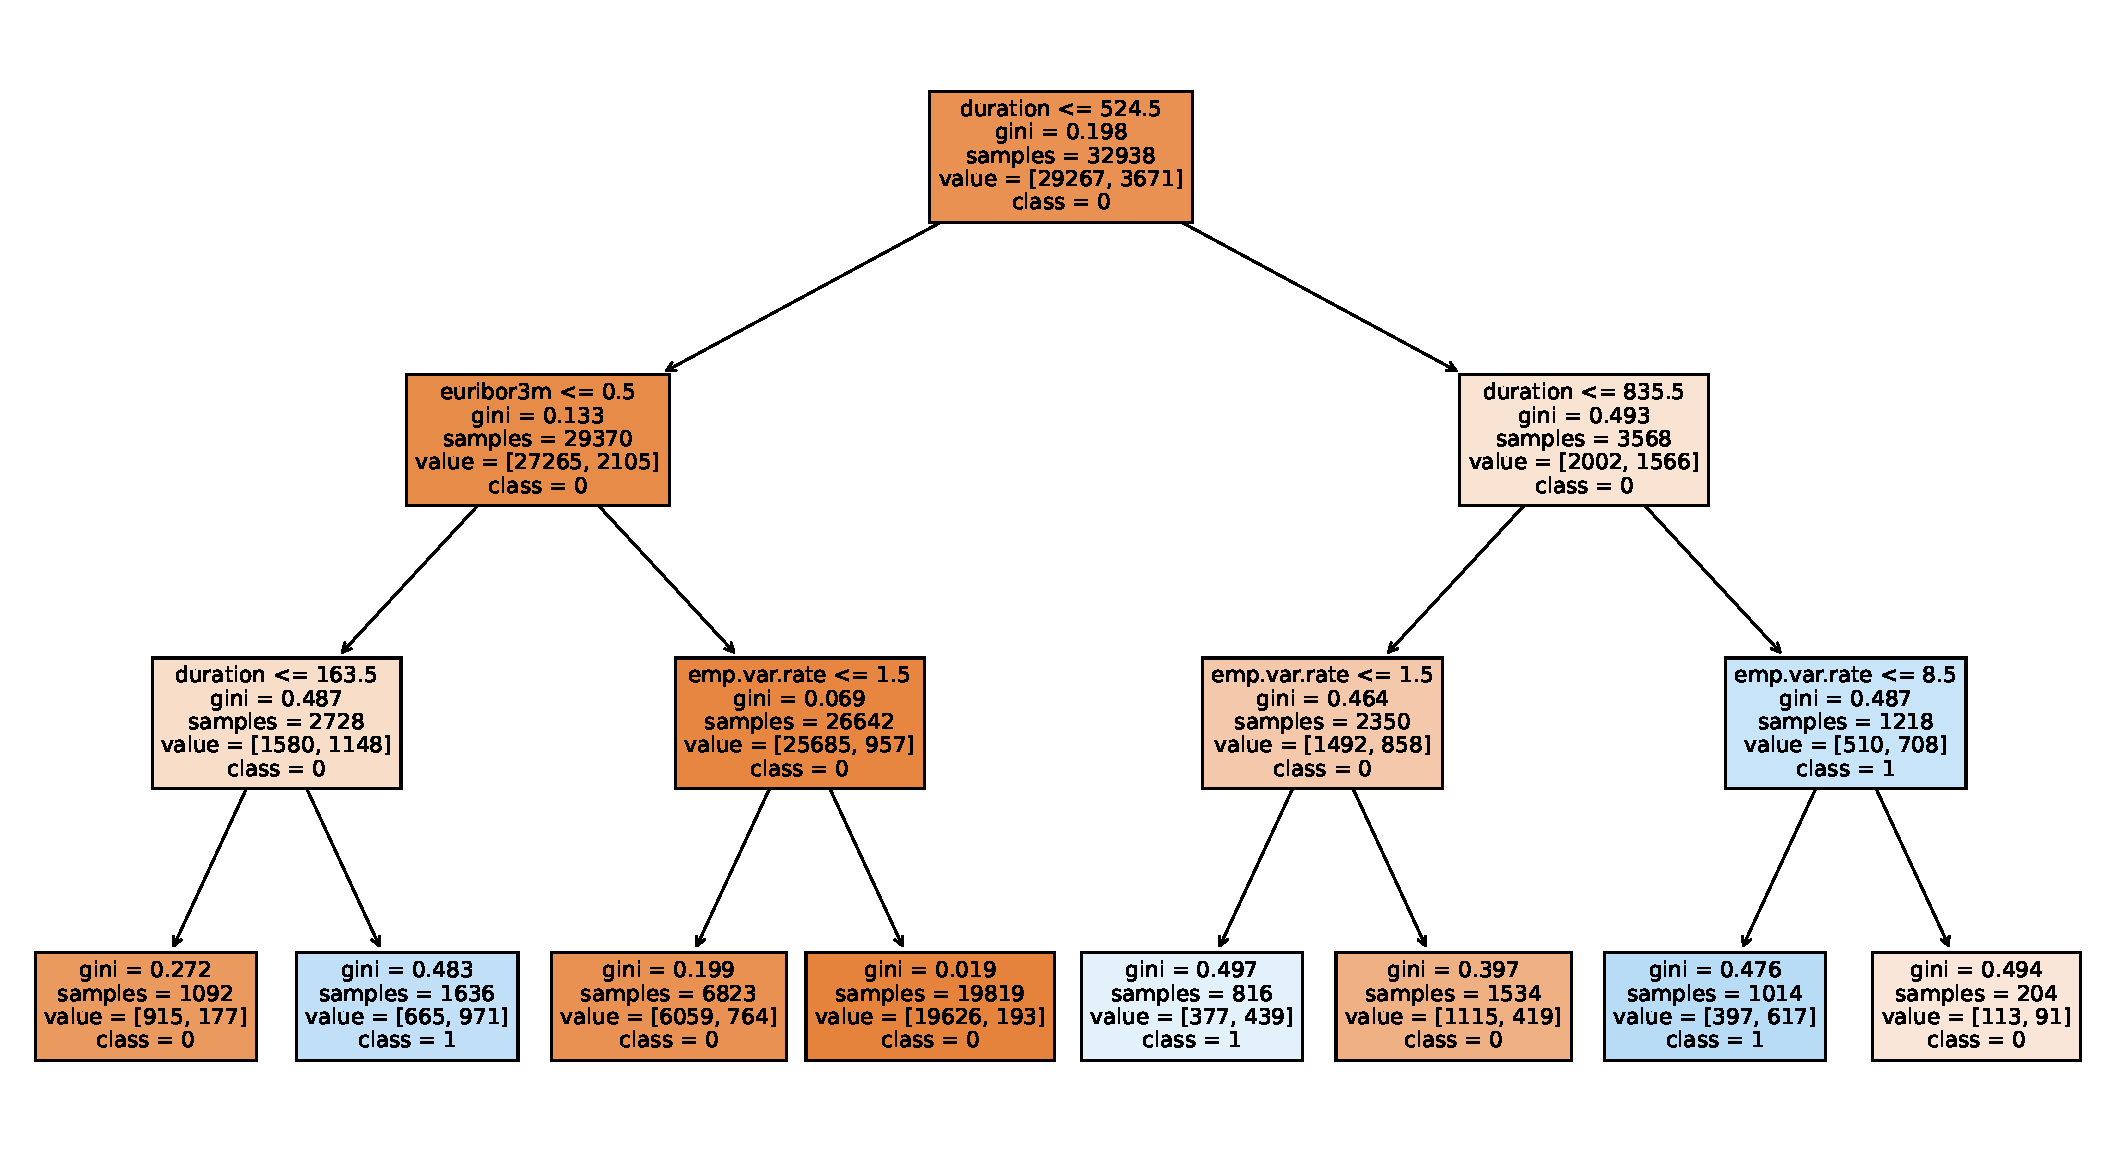
\includegraphics[width=\textwidth]{plot/classification/decision_tree.pdf}
        \caption{Decision Tree}
        \label{fig:decision_tree}
    \end{figure}

    
    % \newpage
    \noindent
    \textbf{Decision Rules} \\
    {
% \begin{lstlisting}[language = Python]
% r = tree.export_text(dt, feature_names=list(dataset_prepared.columns))
% print(r)

% |--- nr.employed <= 5087.65
% |   |--- duration <= 162.50
% |   |   |--- duration <= 123.50
% |   |   |   |--- class: 0
% |   |   |--- duration >  123.50
% |   |   |   |--- class: 0
% |   |--- duration >  162.50
% |   |   |--- pdays <= 15.50
% |   |   |   |--- class: 1
% |   |   |--- pdays >  15.50
% |   |   |   |--- class: 1
% |--- nr.employed >  5087.65
% |   |--- duration <= 524.50
% |   |   |--- cons.conf.idx <= -46.65
% |   |   |   |--- class: 0
% |   |   |--- cons.conf.idx >  -46.65
% |   |   |   |--- class: 0
% |   |--- duration >  524.50
% |   |   |--- duration <= 835.50
% |   |   |   |--- class: 0
% |   |   |--- duration >  835.50
% |   |   |   |--- class: 1
% \end{lstlisting}
        
    }

    \setcounter{magicrownumbers}{0}
    \newcommand\rules{\stepcounter{magicrownumbers}\arabic{magicrownumbers}}
    \begin{tabular}{r l}
        R\rules & If \texttt{duration} $<$= 524.5 and \texttt{euribor3m} $<$= 0.5 and \texttt{duration} $<$= 163.5, then \texttt{y} = 0 \\
        & Gini = 0.272, Support = 0.0332, Confidence = 0.8379, Capture = 0.0313 \\
        
        R\rules & If \texttt{duration} $<$= 524.5 and \texttt{euribor3m} $<$= 0.5 and \texttt{duration} $>$ 163.5, then \texttt{y} = 1 \\
        & Gini = 0.483, Support = 0.0497, Confidence = 0.5935, Capture = 0.2645 \\
        
        R\rules & If \texttt{duration} $<$= 524.5 and \texttt{euribor3m} $>$ 0.5 and \texttt{emp.var.rate} $<$= 1.5, then \texttt{y} = 0 \\
        & Gini = 0.199, Support = 0.2071, Confidence = 0.8880, Capture = 0.2070 \\
        
        R\rules & If \texttt{duration} $<$= 524.5 and \texttt{euribor3m} $>$ 0.5 and \texttt{emp.var.rate} $>$ 1.5, then \texttt{y} = 0 \\
        & Gini = 0.019, Support = 0.6017, Confidence = 0.9902, Capture = 0.6706\\
        
        R\rules & If \texttt{duration} $>$ 524.5 and \texttt{duration} $<$= 835.5 and \texttt{emp.var.rate} $<$= 1.5, then \texttt{y} = 1 \\
        & Gini = 0.497, Support = 0.0247, Confidence = 0.5380, Capture = 0.1196 \\
        
        R\rules & If \texttt{duration} $>$ 524.5 and \texttt{duration} $<$= 835.5 and \texttt{emp.var.rate} $>$ 1.5, then \texttt{y} = 0 \\
        & Gini = 0.397, Support = 0.0466, Confidence = 0.7269, Capture = 0.0381 \\
        
        R\rules & If \texttt{duration} $>$ 524.5 and \texttt{duration} $>$ 835.5 and \texttt{emp.var.rate} $<$= 8.5, then \texttt{y} = 1 \\
        & Gini = 0.476, Support = 0.0308, Confidence = 0.6085, Capture = 0.1681 \\
        
        R\rules & If \texttt{duration} $>$ 524.5 and \texttt{duration} $>$ 835.5 and \texttt{emp.var.rate} $>$ 8.5, then \texttt{y} = 0 \\
        & Gini = 0.494, Support = 0.0062, Confidence = 0.5539, Capture = 0.0039 \\
        
    \end{tabular} \\ \\
    As the maximum depth is set to be only 3, there are only 8 rules, and quite a few redundant leafs, e.g., R3 and R4 could be combined into one rule: If \texttt{duration} $<$= 524.5 and \texttt{euribor3m} $>$ 0.5, then \texttt{y} = 0
    
    \newpage
    \subsection{Random Forest} \label{random_forest}
    Again, the depth of decision trees are set to be 3, a simplified random forest is as followed:
    
% \begin{lstlisting}[language = Python]
% # Set max_depth = 3 to keep the size of the tree small for ploting graph
% rf = RandomForestClassifier(max_depth = 3, n_estimators = 10,
%                             random_state = random_state)
% rf.fit(x_train, y_train)

% # Plot 3 trees of the Forest
% fig, axes = plt.subplots(nrows = 3, ncols = 1, figsize = (10,15), dpi = 100)
% for index in range(0, 3):
%     plt.figure(figsize = (10,5))
%     tree.plot_tree(rf.estimators_[index], feature_names = dataset_prepared.columns,
%                       class_names = ["0", "1"], filled = True, ax = axes[index])
%     axes[index].set_title('Estimator: ' + str(index), fontsize = 11)
% \end{lstlisting}

    \begin{figure}[!ht]
        \centering
        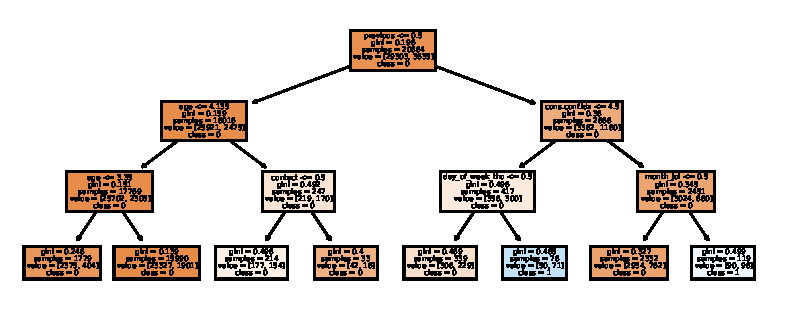
\includegraphics[width = \textwidth]{plot/classification/random_forest0.pdf}
        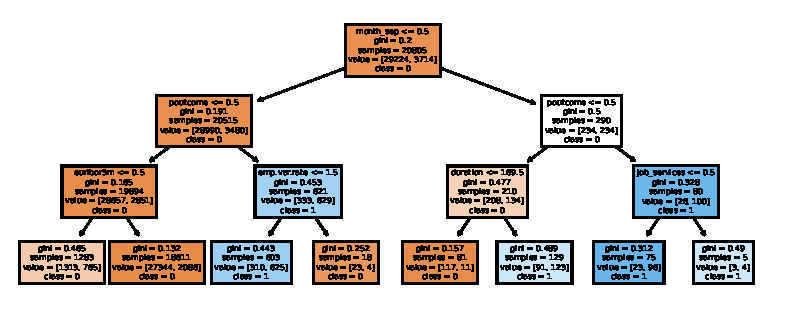
\includegraphics[width = \textwidth]{plot/classification/random_forest1.pdf}
        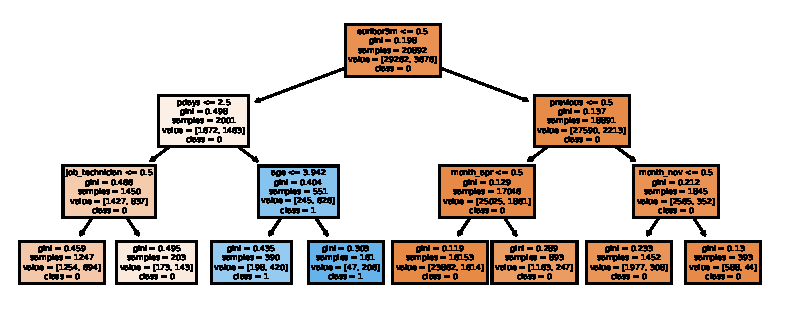
\includegraphics[width = \textwidth]{plot/classification/random_forest2.pdf}
        \caption{Random Forest}
        \label{fig:random_forest}
    \end{figure}
    
    \newpage
    \noindent
    In this simplified random forest, we obtain 10 decision trees (only 3 were printed above), then the prediction is obtained by the majority vote in the case of classification.
    
    
    \subsection{Logistic Regression} \label{logistic_regression}
    Since random forest is expansion of decision tree, we also include logistic regression to compare with former two models. Notice that plotting the logistic regression logit plot requires extremely long time for plotting ten of thousands of points, so we only use \texttt{duration} as explanatory variable to demonstrate in plot.
    
    
    
    \subsection{Cross Validation and Grid Search Procedures}
    To optimize our prediction model, we use cross validation and grid search to find the optimized parameters. This step is implemented using \texttt{Pipeline} and \texttt{GridSearchCV} from \texttt{sklearn}. The training accuracy rate, testing accuracy rate and computation time are calculated base on the best model under grid search. \\
% \begin{lstlisting}[language = Python]
% # RandomForestClassifier
% RandomForest = Pipeline([('rf', RandomForestClassifier(n_jobs=-1,random_state=random_state))])

% # DecisionTreeClassifier
% DecisionTree = Pipeline([('dt', tree.DecisionTreeClassifier(max_features='auto',random_state=random_state))])

% # Set number of Cross Validation
% cv = StratifiedKFold(shuffle=True, n_splits=5,random_state=random_state)

% # Set parameters for RandomForestClassifier and DecisionTreeClassifier
% rf_params = [{  'rf__criterion': ['entropy'],
%                 'rf__min_samples_leaf': [80, 100],
%                 'rf__max_depth': [25, 27],
%                 'rf__min_samples_split': [3, 5],
%                 'rf__n_estimators' : [60, 70]}]

% dt_params = [{  'dt__max_depth': [8, 10],
%                 'dt__min_samples_leaf': [1, 3, 5, 7]}]

% #  Set parameters for Grid Search of RandomForestClassifier and DecisionTreeClassifier
% gs_rf = GridSearchCV(RandomForest, param_grid=rf_params,
%                      scoring='accuracy', cv=cv)

% gs_dt = GridSearchCV(DecisionTree, param_grid=dt_params,
%                      scoring='accuracy', cv=cv)

% # Models used
% model_used = [gs_rf, gs_dt]
% model_name = { 0:'RandomForest', 1:'DecisionTree'}

% # Set temp
% acc_rate = {}
% auc_rate = {}
% models = []
% time_used={}

% # Record the time used, accuracy rate and ROC rate
% for index, model in enumerate(model_used):
%         start = time.time()
%         print('Using {} model'.format(model_name[index]))
%         model.fit(x_train, y_train)
%         print('training accuracy rate is {}'.format(model.best_score_))
%         auc = roc_auc_score(y_test, model.predict_proba(x_test)[:,1])
%         print('testing accuracy rate is {} and ROC_AUC is {}'.format(model.score(x_test, y_test),auc))
%         end = time.time()
%         print('It requires {} sec to compute'.format(round(end - start, 2)))
%         print()
        
%         models.append(model.best_estimator_)
%         acc_rate[index] = model.score(x_test, y_test)
%         auc_rate[index] = auc
%         time_used[index] = round(end - start, 2)
% \end{lstlisting}
    % \noindent
    
    \noindent
    \textbf{Output:} (refer to source code)
    
    \noindent
    \texttt{Using RandomForest model \\
    training accuracy rate is 0.9061448004270909 \\
    testing accuracy rate is 0.9014814215170404 and ROC\_AUC is 0.9329564140543615 \\
    It requires 64.35 sec to compute \\
    \\
    Using DecisionTree model \\
    training accuracy rate is 0.9045141750723605 \\
    testing accuracy rate is 0.8998623816077066 and ROC\_AUC is 0.8852839212278664 \\
    It requires 1.88 sec to compute}
    

    \subsection{Comparison of Performance of Random Forest and Decision Tree}
    
    \subsubsection{Accuracy Rate, ROC rate and Computation Time}
% \begin{lstlisting}[language = Python]
% pd.DataFrame(
%     list(zip(model_name.values(), acc_rate.values(), auc_rate.values(), time_used.values())), 
%     columns = ['Model_used', 'Testing_accuracy_rate','Testing_ROC_rate','Time_used']
% )
% \end{lstlisting}
%     \noindent
    \begin{table}[ht]
        \centering
        \begin{tabular}{llrrr}
            {} &    Model\_used &  Testing\_accuracy\_rate &  Testing\_ROC\_rate &  Time\_used \\
            \hline \hline
            0 &  RandomForest &               0.899818 &          0.935413 &      84.41 \\
            1 &  DecisionTree &               0.894839 &          0.905776 &       2.09 \\
        \end{tabular}
        \caption{Accuracy Rate, ROC rate and Computation Time}
        \label{tab:comparison}
    \end{table}

    
    \subsubsection{ROC Graph}
% \begin{lstlisting}[language = Python]
% def plot_ROC(fpr, tpr, threshold,model):
%     trace0 = go.Scatter(x=fpr[0], y=tpr[0], text=threshold[0], fill='tozeroy', name='ROC Curve of {} '.format(model[0]))
%     trace1 = go.Scatter(x=fpr[1], y=tpr[1], text=threshold[1], fill='tozeroy', name='ROC Curve of {} '.format(model[1]))
%     trace2 = go.Scatter(x=[0,1], y=[0,1], line={'color': 'black', 'width': 1, 'dash': 'dash'}, name='Baseline')
%     data = [trace0, trace1, trace2]
    
%     layout = go.Layout(title='ROC Curve', xaxis={'title': 'False Positive Rate'}, 
%                       yaxis={'title': 'True Positive Rate'})
%     fig = go.Figure(data, layout)
%     fig.write_image("../../plot/classification/roc.pdf")
%     fig.show()

% fpr, tpr, threshold = np.transpose([
%     roc_curve(y_test, models[0].predict_proba(x_test)[:,1]), 
%     roc_curve(y_test, models[1].predict_proba(x_test)[:,1])
% ])

% plot_ROC(fpr = fpr, tpr = tpr, threshold = threshold, model = ["Random Forest", "Decision Tree"])
% \end{lstlisting}
%     \noindent
    
    \begin{figure}[H]
        \centering
        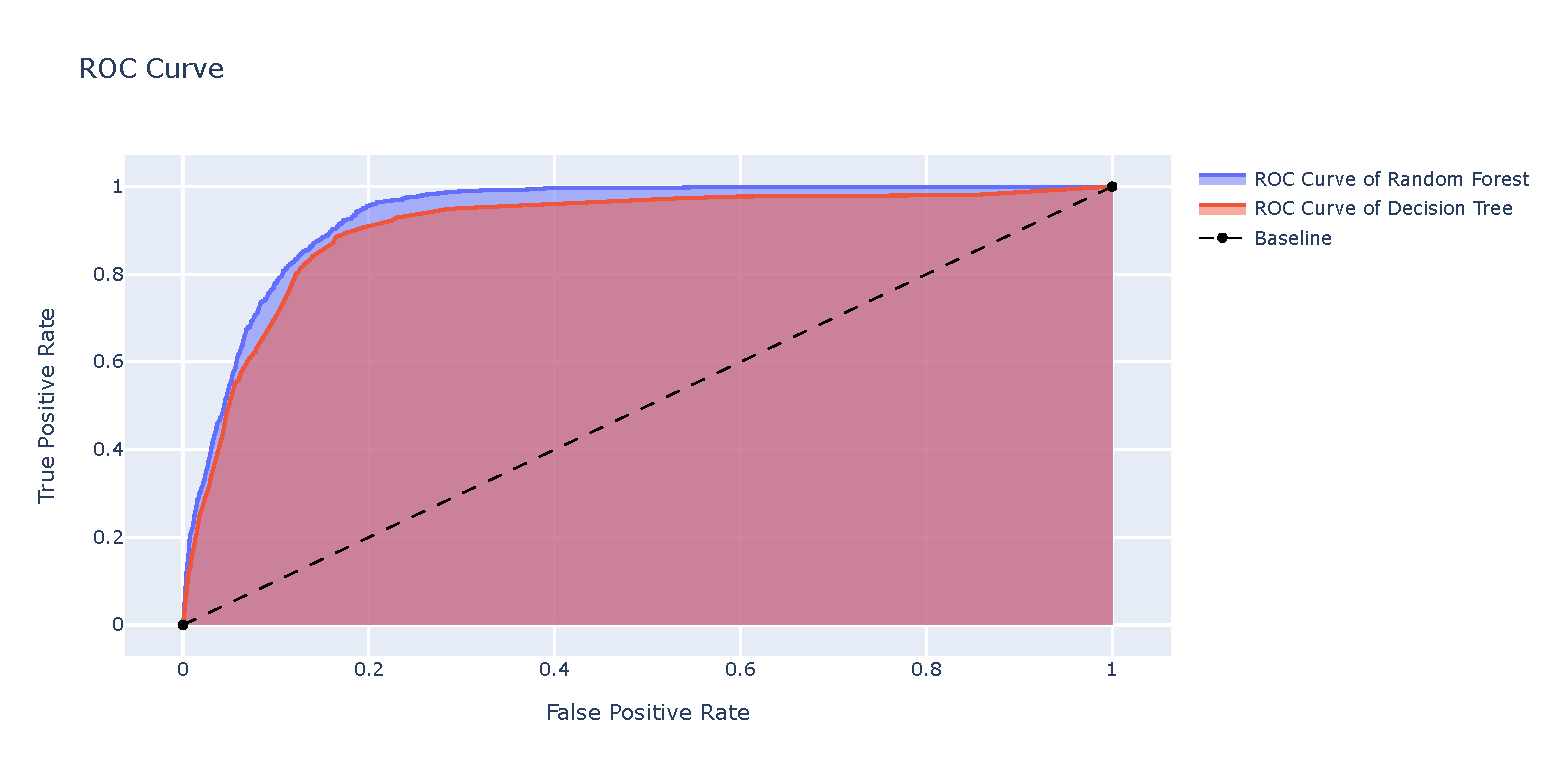
\includegraphics[width = \textwidth]{plot/classification/roc.pdf}
        \caption{ROC Graph}
        \label{fig:roc}
    \end{figure}

    
    
    \subsection{Conclusion}
    In terms of performance, random forest has a higher accuracy rate and ROC rate (0.8998, 0.9354) comparing to that of decision tree (0.8948, 0.9058). The accuracy rate are similar in both method. \\
    Speaking of computation time, decision tree requires shorter time ($\sim$ 2.09s), while random forest requires 40 times longer in computation ($\sim$ 84.41s), there is a huge difference. \\
    Our group believe that random forest performs better than decision tree in this case. Since this dataset contains around 40,000 rows, the required computation time is around 80s, which is reasonable. Also, random forest has a significantly better ROC rate.
    
    
    \newpage
    \section{Bibliography}
    \bibliographystyle{unsrt}
    % \bibliographystyle{plain} % We choose the "plain" reference style
    \bibliography{refs} % Entries are in the refs.bib file

\end{document}